\documentclass[a4paper,12pt]{article}
\usepackage[english]{babel}
\usepackage[utf8]{inputenc}

%
% For alternative styles, see the biblatex manual:
% http://mirrors.ctan.org/macros/latex/contrib/biblatex/doc/biblatex.pdf
%
% The 'verbose' family of styles produces full citations in footnotes, 
% with and a variety of options for ibidem abbreviations.
%
\usepackage{graphicx}
\usepackage{csquotes}
\usepackage[style=verbose-ibid,backend=bibtex]{biblatex}
\bibliography{sample}

\title{Markovian Approach to Positive-only Problems}

\author{Shayan Amani}

\begin{document}
\maketitle

\section{Preliminaries}


\section{Methodology}
These two methods have distinct approach in distribution modeling. MaxLike estimates probability of occurrence, while MaxEnt estimates a relative suitability index. According to Fitzpatrick et al. (2013) there is no apparent correlation or proximity between MaxEnt’s indices and probability of occurrence. By default, the MaxEnt algorithm assumes a baseline species prevalence of 0.5 \cite{Phillips2008}. Therefore, MaxEnt assigns occurrence probability of 0.5 to most occurrence locations

\section{Case Study}

% 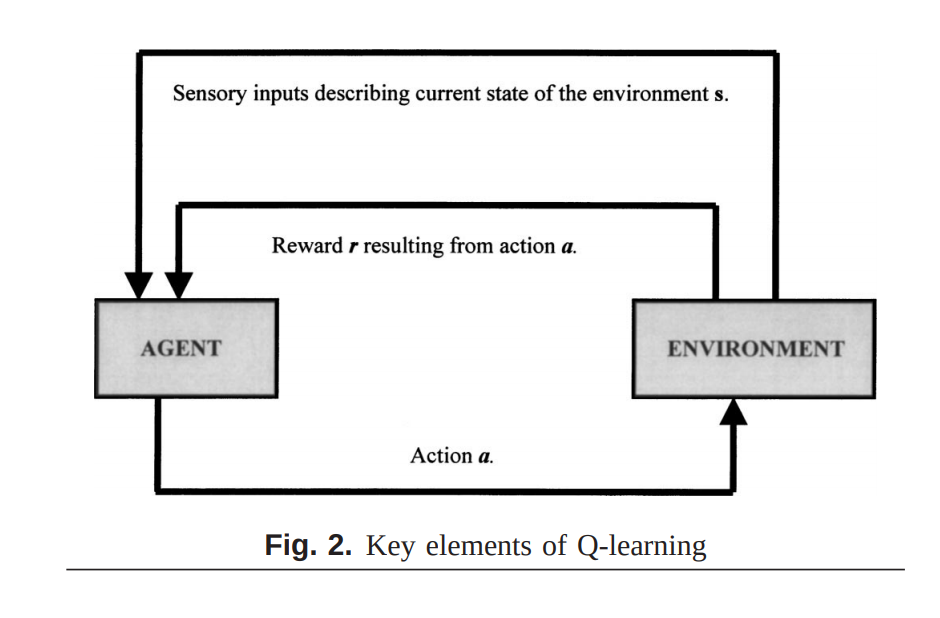
\includegraphics[width=1\columnwidth]{elements.png}



% This is an example citation \autocite{ginsberg}.
% \lipsum[1] % dummy text

% This is another example citation \autocite{brassard}.
% \lipsum[2] % dummy text

% This is a repeated citation \autocite{brassard}.
% \lipsum[3] % dummy text

% This is another example citation \autocite{adorf}.
% \lipsum[4] % dummy text 

\end{document}